\documentclass{beamer}
%
% Choose how your presentation looks.
%
% For more themes, color themes and font themes, see:
% http://deic.uab.es/~iblanes/beamer_gallery/index_by_theme.html
%
\mode<presentation>
{
  \usetheme{default}      % or try Darmstadt, Madrid, Warsaw, ...
  \usecolortheme{default} % or try albatross, beaver, crane, ...
  \usefonttheme{default}  % or try serif, structurebold, ...
  \setbeamertemplate{navigation symbols}{}
  \setbeamertemplate{caption}[numbered]
}

\makeatletter
\def\maxwidth{ %
	\ifdim\Gin@nat@width>\linewidth
	\linewidth
	\else
	\Gin@nat@width
	\fi
}
\makeatother

\definecolor{fgcolor}{rgb}{0.345, 0.345, 0.345}
\newcommand{\hlnum}[1]{\textcolor[rgb]{0.686,0.059,0.569}{#1}}%
\newcommand{\hlstr}[1]{\textcolor[rgb]{0.192,0.494,0.8}{#1}}%
\newcommand{\hlcom}[1]{\textcolor[rgb]{0.678,0.584,0.686}{\textit{#1}}}%
\newcommand{\hlopt}[1]{\textcolor[rgb]{0,0,0}{#1}}%
\newcommand{\hlstd}[1]{\textcolor[rgb]{0.345,0.345,0.345}{#1}}%
\newcommand{\hlkwa}[1]{\textcolor[rgb]{0.161,0.373,0.58}{\textbf{#1}}}%
\newcommand{\hlkwb}[1]{\textcolor[rgb]{0.69,0.353,0.396}{#1}}%
\newcommand{\hlkwc}[1]{\textcolor[rgb]{0.333,0.667,0.333}{#1}}%
\newcommand{\hlkwd}[1]{\textcolor[rgb]{0.737,0.353,0.396}{\textbf{#1}}}%

\usepackage{framed}
\makeatletter
\newenvironment{kframe}{%
	\def\at@end@of@kframe{}%
	\ifinner\ifhmode%
	\def\at@end@of@kframe{
		\begin{minipage}}%

	\end{minipage}{\columnwidth}%
	\fi\fi%
	\def\FrameCommand##1{\hskip\@totalleftmargin \hskip-\fboxsep
		\colorbox{shadecolor}{##1}\hskip-\fboxsep
		% There is no \\@totalrightmargin, so:
		\hskip-\linewidth \hskip-\@totalleftmargin \hskip\columnwidth}%
	\MakeFramed {\advance\hsize-\width
		\@totalleftmargin\z@ \linewidth\hsize
		\@setminipage}}%
{\par\unskip\endMakeFramed%
	\at@end@of@kframe}
\makeatother

\newenvironment{knitrout}{}{} % an empty environment to be redefined in TeX
\usepackage[english]{babel}
\usepackage[utf8x]{inputenc}
\usepackage{alltt}
\usepackage{apacite}
\usepackage{setspace}
\usepackage{float}
\usepackage{framed}


\title[]{Momentum Investment Strategies In the MENA Financial Markets}
\author{Amine Karmouche}
\institute{Al Akhawayn Unievrsity in Ifrane}
\date{June 3rd, 2015}

\begin{document}

\begin{frame}
  \titlepage
\end{frame}

% Uncomment these lines for an automatically generated outline.
%\begin{frame}{Outline}
%  \tableofcontents
%\end{frame}
\section{Outline}
\begin{frame}{Outline}
	\begin{itemize}
			\item Introduction \& Background
			\item Literature Review
			\item Contribution to existing research
			\item Data and Methodology
			\item Empirical Results and Managerial implications
			\item Conclusions and Future Work
	\end{itemize}
\end{frame}

\section{Introduction}
\begin{frame}{Introduction and Background}
	\begin{itemize}
		\item Elimination of some barriers to entry for investors
		\item Openness to competition
		\item Market Potential not scrutinized enough
		\item Presence of diversification potential
	\end{itemize}
\end{frame}

\section{Literature Review}
\begin{frame}{Literature Review}
	\begin{itemize}
		\item Modern Finance Theory
			%\subitem Markowicz(1952) Fama 
		\item Behavioral Finance Theory
			%\subitem Kahneman and Tversky (1979) 
			%\subitem Shefrin and Statman (1985)
			%\subitem Barberis, Shleifer, and Vishny (1998),
		\item Portfolio Management Theory
%			\subitem Markowitz (1952)
%			\subitem Brennan \& Xia (2001) tactical
%			\subitem Jegadeesh \& Titman (1993) momentum
		\item The MENA Financial Markets
%			\subitem Darrat et al. (2000) integration
%			\subitem Assaf (2003) decrease in integration 
%			\subitem Lagoarde-Segot and Lucey (2007) contruscted a portfolio
	\end{itemize}
\end{frame}

\section{Contribution}
\begin{frame}{Contribution to existing Research}
	\begin{itemize}
\item Ejaz and Polak (2015)
\item Extended data set
\item Applies the methodology
\item Extends Anomaly
\item Confirms
	\end{itemize}
\end{frame}

\section{Data}
\begin{frame}{Data}
	\begin{itemize}
		\item Thomson Reuters
		\item Daily closing prices of MENA stock market indices from the years 1998 to 2014
		\item Morocco, Tunisia, Egypt, Saudi Arabia, Lebanon, Jordan, and Turkey
		\item MASI / TUNINDEX / EGX 30 Index / Tadawul (TASI) / BLOM / ASE Index / XU100  
	\end{itemize}
\end{frame}

\begin{frame}{Data (cont'd)}
	\begin{itemize}
		\item Converted to USD using the daily spot rate
		\item VFISX Exchange Traded Fund will be used as a proxy for cash
		\item Data was cleaned and aligned 		
	\end{itemize}
\end{frame}

\begin{frame}{Data (cont'd)}
	Descriptive Statistics
	\begin{itemize}
		\item Insert statistics here!
	\end{itemize}
\end{frame}

% Methodology Section 
\section{Methodology}
\begin{frame}{Methodology}
	\begin{itemize}
		\item A portion of the historical data, referred to as "in-sample" will be used to identify the best trading model to apply to the "out of sample data". 
		\item The parameters to be set after backtesting the strategy are: 
%			\subitem Rebalancing frequency (set to 1 month)
%			\subitem Lookback period
	\end{itemize}
\end{frame}

\begin{frame}{Methodology cont'd}
	\begin{itemize}
		\item Formulas for price and return momentum and others using Latex 
	\end{itemize}
	
	$$S_n = \frac{X_1 + X_2 + \cdots + X_n}{n}
	= \frac{1}{n}\sum_{i}^{n} X_i$$
	denote their mean. Then as $n$ approaches infinity, the random variables $\sqrt{n}(S_n - \mu)$ converge in distribution to a normal $\mathcal{N}(0, \sigma^2)$.
	
\end{frame}

\begin{frame}{Methodology}
	Flowchart
	\begin{itemize}
		\item Computing the assets returns for a certain lookback period
		\item Ranking the assets based on their return momentum and selecting the
		best N
		\item The ones with a negative price momentum will be sold and replaced
		by the risk-free security, i.e the VFISX ETF.
		\item Other assets not retained will be sold
		\item  This winning portfolio will be held during the portfolio holding period
	\end{itemize}
\end{frame}

\begin{frame}{Methodology: Performance Metrics}
	Metrics
	\begin{itemize}
		\item Annualized return
		\item Max Drawdown
		\item Annualized Sharpe Ratio
		\item Calmar Ratio
	\end{itemize}
	Benchmark
	\begin{itemize}
		\item S\&P 500 Buy and Hold
	\end{itemize}
\end{frame}

\begin{frame}{Backtesting }
	Periods (insert timeline)
	\begin{itemize}
		\item In-sample: 1998-2004
		\item Out-of-Sample 2005-2014
	\end{itemize}
	In-Sample
	\begin{itemize}
		\item Number of winning assets 
		\item Rebalancing frequency
		\item Lookback period please highlight!
	\end{itemize}
	Out-of-sample
	\begin{itemize}
		\item backtesting strategy will applied to the data spanning from 2005 to 2014.
	\end{itemize}
\end{frame}

\begin{frame}{Backtesting Set-up}
	Platform
	\begin{itemize}
		\item R programming language was used to simulate the trading strategy. 
		\item The quantitative finance packages are a benchmark in trading practice 
		\item FinancialInstrument PerformanceAnalytics quantmod
	\end{itemize}
	Risk-free asset
	\begin{itemize}
		\item Risk free asset is VFISX fund which is used as a proxy for cash and cash equivalents.	
	\end{itemize}
\end{frame}

\section{Empirical Results}
\begin{frame}{Empirical Results}
	In-sample performance
	\begin{itemize}
		\item Using 1, 3, 6, and 9 months as lookback formation periods
		
		
	\end{itemize}
\end{frame}

\begin{frame}{In-sample Performance}
	\begin{itemize}
		\item Formation period: 3 months
		\item Holding period: 1 month
	\end{itemize}
	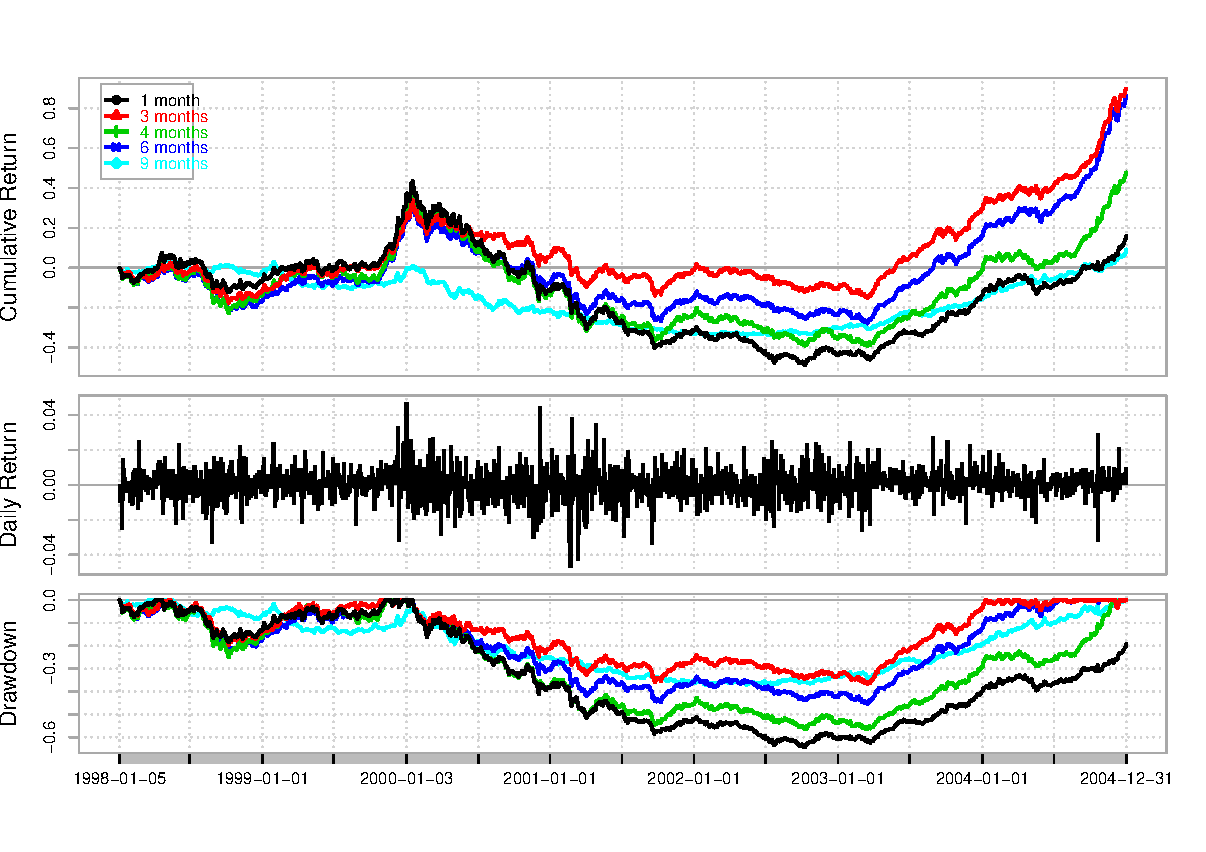
\includegraphics[width=\maxwidth]{figures/FinalIn}
\end{frame}

\begin{frame}{In-sample Performance cont'd}
	\begin{itemize}
		\item table
	\end{itemize}
	
	\begin{table}
		\centering
		\begin{tabular}{l|r}
			Item & Quantity \\\hline
			Widgets & 42 \\
			Gadgets & 13
		\end{tabular}
		\caption{\label{tab:widgets}An example table.}
	\end{table}
\end{frame}

\begin{frame}{Out-of-Sample performance}
	\begin{itemize}
		\item here
	\end{itemize}
	
	\begin{figure}
		\includegraphics[width=\maxwidth]{figures/FinalOut}
		\caption{\label{fig:your-figure}Out of sample}
	\end{figure}
\end{frame}

\section{Conclusion}
\begin{frame}{Conclusion and Future Work}
	\begin{itemize}
		\item
	\end{itemize}
\end{frame}
\end{document}
